\documentclass{report}

\usepackage[T2A]{fontenc}
\usepackage[utf8]{luainputenc}
\usepackage[english, russian]{babel}
\usepackage[pdftex]{hyperref}
\usepackage[14pt]{extsizes}
\usepackage{listings}
\usepackage{color}
\usepackage{geometry}
\usepackage{enumitem}
\usepackage{multirow}
\usepackage{graphicx}
\usepackage{indentfirst}
\usepackage{amsmath}


\geometry{a4paper,top=2cm,bottom=3cm,left=2cm,right=1.5cm}
\setlength{\parskip}{0.5cm}
\setlist{nolistsep, itemsep=0.3cm,parsep=0pt}

\lstset{language=C++,
		basicstyle=\footnotesize,
		keywordstyle=\color{blue}\ttfamily,
		stringstyle=\color{red}\ttfamily,
		commentstyle=\color{green}\ttfamily,
		morecomment=[l][\color{magenta}]{\#}, 
		tabsize=4,
		breaklines=true,
  		breakatwhitespace=true,
  		title=\lstname,       
}

\makeatletter
\renewcommand\@biblabel[1]{#1.\hfil}
\makeatother

\begin{document}

\begin{titlepage}

\begin{center}
Министерство науки и высшего образования Российской Федерации
\end{center}

\begin{center}
Федеральное государственное автономное образовательное учреждение высшего образования \\
Национальный исследовательский Нижегородский государственный университет им. Н.И. Лобачевского
\end{center}

\begin{center}
Институт информационных технологий, математики и механики
\end{center}

\vspace{4em}

\begin{center}
\textbf{\LargeОтчет по лабораторной работе} \\
\end{center}
\begin{center}
\textbf{\Large«Сортировка Шелла с простым слиянием»} \\
\end{center}

\vspace{4em}

\newbox{\lbox}
\savebox{\lbox}{\hbox{text}}
\newlength{\maxl}
\setlength{\maxl}{\wd\lbox}
\hfill\parbox{7cm}{
\hspace*{5cm}\hspace*{-5cm}\textbf{Выполнил:} \par студент группы 381806-1 \par Стрельцова Я. Д.\par
\par
\hspace*{5cm}\hspace*{-5cm}\textbf{Проверил:}\par доцент кафедры МОСТ, \par кандидат технических наук \par Сысоев А. В.\par
}

\vspace{\fill}

\begin{center} Нижний Новгород \par 2021 \end{center}

\end{titlepage}

\setcounter{page}{2}

% Содержание
\tableofcontents
\newpage

% Введение
\section*{Введение}
\addcontentsline{toc}{section}{Введение}
Сортировка Шелла была названа в честь ее изобретателя – Дональда Шелла, который опубликовал этот алгоритм в 1959 году. Общая идея состоит в сравнении на начальных стадиях сортировки пар значений, расположенных достаточно далеко друг от друга в упорядочиваемом наборе данных. Такая модификация метода сортировки позволяет быстро переставлять далекие неупорядоченные пары значений. Эффективность сортировки Шелла в определённых случаях обеспечивается тем, что элементы «быстрее» встают на свои места (в простых методах сортировки, например, пузырьковой, каждая перестановка двух элементов уменьшает количество инверсий в списке максимум на 1, а при сортировке Шелла это число может быть больше).

Невзирая на то, что сортировка Шелла во многих случаях медленнее, чем быстрая сортировка, она имеет ряд преимуществ:
\begin{itemize}
  \item отсутствие потребности в памяти под стек;
  \item отсутствие деградации при неудачных наборах данных — быстрая сортировка легко деградирует до O(n²), что хуже, чем худшее гарантированное время для сортировки Шелла.
\end{itemize}
    
Т.к. сортировка Шелла представляет собой алгоритм, требующий многократных обходов сортируемого диапазона, то с увелечением числа сортируемых объектов, увеличивается и время, требуемое для сортировки. Запуск на нескольких процессорах вычислительного оборудования может помочь уменьшить затраты времени на сортировку.

\newpage

% Постановка задачи
\section*{Постановка задачи}
\addcontentsline{toc}{section}{Постановка задачи}
В рамках лабораторной работы необходимо реализовать алгоритм сортировки Шелла с простым слиянием, проверить корректность работы алгоритмов, провести вычислительные эксперименты и сравнить эффективность последовательной и параллельной реализаций.

Работа должна содержать следующие модули:
\begin{itemize}
  \item последовательная реализация;
  \item реализация с помощью OpenMP;
  \item реализация с помощью TBB.
\end{itemize}

Для проверки корректности работы алгоритмов используется Google Testing Framework.
\newpage

% Описание алгоритма
\section*{Описание алгоритма}
\addcontentsline{toc}{section}{Описание алгоритма}
Идея метода заключается в сравнение разделенных на группы элементов последовательности, находящихся друг от друга на некотором расстоянии. Изначально это расстояние равно d или N/2, где N — общее число элементов. На первом шаге каждая группа включает в себя два элемента расположенных друг от друга на расстоянии N/2; они сравниваются между собой, и, в случае необходимости, меняются местами. На последующих шагах также происходят проверка и обмен, но расстояние d сокращается на d/2, и количество групп, соответственно, уменьшается. Постепенно расстояние между элементами уменьшается, и на d=1 проход по массиву происходит в последний раз.

Далее, на примере последовательности целых чисел, показан процесс сортировки массива методом Шелла. Для удобства и наглядности, элементы одной группы выделены одинаковым цветом.
\begin{table}[!h]
\centering
\begin{tabular}{ | c | l | l | l  | l | l | l | l | l | l | l |}
\hline
Исходный массив & 5 & 3 & 8 & 0 & 7 & 4 & 9 & 1 & 6 & 2\\ \hline
d = 5 &4&\textcolor{red}{3}&\textcolor{blue}{1}&\textcolor{green}{0}&\textcolor{magenta}{2}&5&\textcolor{red}{9}&\textcolor{blue}{8}&\textcolor{green}{6}&\textcolor{magenta}{7}\\ \hline
d = 2 &1&\textcolor{red}{0}&2&\textcolor{red}{3}&4&\textcolor{red}{5}&6&\textcolor{red}{7}&9&\textcolor{red}{8}\\ \hline
d = 1 & 0 & 1 & 2 & 3 & 4 & 5 & 6 & 7 & 8 & 9\\ \hline
\end{tabular}
\caption{Пример сортировки Шелла}
\end{table}

Первое значение, соответствующее расстоянию d равно 10/2=5. На каждом шаге оно уменьшается вдвое. Элементы, входящие в одну группу, сравниваются и если значение какого-либо элемента, стоящего левее того с которым он сравнивается, оказывается больше (сортировка по возрастанию), тогда они меняются местами. Так, элементы путем внутригрупповых перестановок постепенно становятся на свои позиции, и на последнем шаге (d=1) сортировка сводится к проходу по одной группе, включающей в себя все N элементов массива. При этом число требуемых обменов оказывается совсем небольшим.

\newpage

% Описание схемы распараллеливания
\section*{Описание схемы распараллеливания}
\addcontentsline{toc}{section}{Описание схемы распараллеливания}

Идея параллельной многопоточной реализации алгоритма Шелла иллюстрируется в таблице, где предполагается использование значений {d = 4; 2; 1}. Каждая строка соответствует подсписку элементов, сортируемых в одном потоке независимо от других элементов массива.

%\begin{figure}[h]
%\center{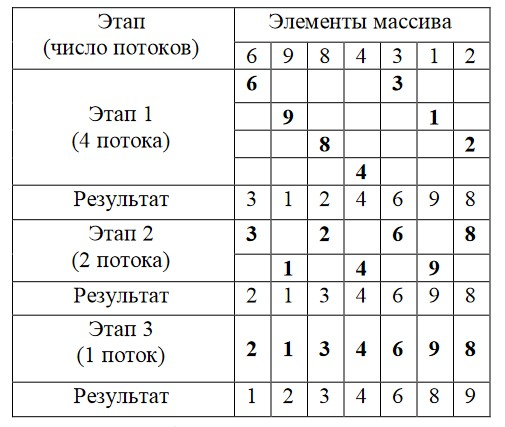
\includegraphics[scale=1.0]{sort_shell2.jpg}}
%\caption{Алгоритм параллельной сортировки Шелла}
%\end{figure}

\begin{center}
\begin{tabular}{| c | c | c | c | c | c | c | c |}\hline
& \multicolumn{7}{c|}{Элементы массива} \\
\cline{2-8}
\raisebox{1.5ex}[0cm][0cm]{Этапы (число потоков)}
& 6 & 9 & 8 & 4 & 3 & 1 & 2 \\ \hline
\hline
\multirow{4}{*}{Этап 1 (4 потока)} & \textbf{6} & & & & \textbf{3} & &  \\ \cline{2-8}
 & & \textbf{9} & & & & \textbf{1} & \\ \cline{2-8}
 & & & \textbf{8} & & & & \textbf{2} \\ \cline{2-8}
 & & & & \textbf{4} & & & \\ \hline
Результат & 3 & 1 & 2 & 4 & 6 & 9 & 8 \\ \hline
 \hline
\multirow{2}{*}{Этап 2 (2 потока)} & \textbf{3} & & \textbf{2} & & \textbf{6} & & \textbf{8} \\ \cline{2-8}
 & & \textbf{1} & & \textbf{4} & & \textbf{9} & \\ \hline
Результат & 2 & 1 & 3 & 4 & 6 & 9 & 8 \\ \hline
 \hline
\multirow{1}{*}{Этап 3 (1 поток)} & \textbf{2} & \textbf{1} & \textbf{3} & \textbf{4} & \textbf{6} & \textbf{9} & \textbf{8} \\ \hline
Результат & 1 & 2 & 3 & 4 & 6 & 9 & 8 \\ \hline
\end{tabular}    
\end{center}

\newpage

% Описание программной реализации
\section*{Описание программной реализации}
\addcontentsline{toc}{section}{Описание программной реализации}
\subsection*{Описание OpenMP-версии}
\addcontentsline{toc}{subsection}{Описание OpenMP-версии}

Параллельная реализация сортировки Шелла с помощью OpenMP представляет собой шаблонную функцию, которая принимает по константной ссылке сортируемый вектор элементов и возвращает по значению отсортированный вектор.
\begin{lstlisting}
template< typename T >
std::vector<T> shell_sort_parallel(const std::vector<T>& vec) {
    if (vec.size() < 1000)
        return shell_sort_sequential(vec);
    std::vector<T> result(vec);
    int d = 4;
    while (d > 0) {
        omp_set_num_threads(d);
#pragma omp parallel
        {
        int tid = omp_get_thread_num();
        for (size_t i = tid; i < result.size(); i += d)
            for (size_t j = i + d; j < result.size(); j += d) {
                if (result[i] > result[j])
                    std::swap(result[i], result[j]);
            }
        }
        d /= 2;
    }
    return result;
}
\end{lstlisting}
С помощью \verb|omp_set_num_threads(d)| задается число потоков равное d. Затем с помощью директивы \verb|#pragma omp parallel| создается параллельная секция, внутри которой вычисляется номер каждого потока и записывается в переменную \verb|tid|. Далее в цикле каждый поток в зависимости от переменной \verb|tid|, сравнивает и сортирует элементы, находящиеся на расстоянии d друг от друга и относящиеся только к его подвектору, независимо от других потков.

\subsection*{Описание TBB-версии}
\addcontentsline{toc}{subsection}{Описание TBB-версии}
Параллельная реализация сортировки Шелла с помощью TBB представляет собой шаблонную функцию, которая принимает по константной ссылке сортируемый вектор элементов и возвращает по значению отсортированный вектор.
\begin{lstlisting}
template< typename T >
std::vector<T> shell_sort_parallel(const std::vector<T>& vec) {
    std::vector<T> result(vec);
    if (vec.size() < 1000)
        return shell_sort_sequential(vec);
    int d = 4;
    while (d > 0) {
        tbb::task_scheduler_init init(d);
        int tid = tbb::task_arena::current_thread_index();
            for (size_t i = tid; i < result.size(); i += d)
                for (size_t j = i + d; j < result.size(); j += d) {
                    if (result[i] > result[j])
                        std::swap(result[i], result[j]);
                }
        init.terminate();
        d /= 2;
    }
    return result;
}
\end{lstlisting}
С помощью \verb|tbb::task_scheduler_init init(d)| создается параллельная секция из d потоков, внутри которой вычисляется номер каждого потока и записывается в переменную \verb|tid|. Далее в цикле каждый поток в зависимости от переменной \verb|tid|, сравнивает и сортирует элементы, находящиеся на расстоянии d друг от друга и относящиеся только к его подвектору, независимо от других потоков.

\newpage

% Результаты экспериментов
\section*{Результаты экспериментов}
\addcontentsline{toc}{section}{Результаты экспериментов}
Вычислительные эксперименты для оценки эффективности параллельного алгоритма сортировки Шелла проводились на оборудовании со следующей аппаратной конфигурацией:

\begin{itemize}
\item Процессор: Intel(R) Core(TM) i5-10210U CPU @ 1.60GHz, 4 ядра;
\item Оперативная память: 8 ГБ;
\item ОС: Microsoft Windows 10 Home 64-bit.
\end{itemize}

В рамках эксперимента было вычислено время работы последовательного и параллельного алгоритмов сортировки Шелла.
В качестве тестируемых данных генерируется вектор случайных чисел типа int от 0 до 100. Запуск производится на 4 потоках.

Результаты экспериментов представлены ниже.
\begin{table}[!h]
\centering
\begin{tabular}{ | l | l | l | l  | l | l | }
\hline
Число элементов  & Последовательно & OpenMP & TBB  \\ \hline
1000  & 0.03737 & 0.02881 &  0.03604 \\ \hline
10000  & 2.95994 & 2.13984 &  2.08730 \\ \hline
100000  & 318.881 & 241.129 &  211.289 \\ \hline
\end{tabular}
\caption{Результаты вычислительных экспериментов}
\end{table}

По данным экспериментов видно, что параллельный алгоритм сортировки Шелла работает быстрее, но ускорение не идеально т.к. начальный размер d равен 4. На больших размерах сортируемого вектора стоит брать значение d равное N/2. Также видно, что на малых размерах вектора эффективнее работает OpenMP-версия, тогда как на больших - TBB.

Для подтверждения корректности в программе представлен набор тестов, разработанных с Google Testing Framework, которые проверяют корректность вычислений путем сравнения векторов, полученных из последовательного и параллельного алгоритмов. Успешное прохождение всех тестов подтверждает корректность работы написанной программы.

\newpage

% Заключение
\section*{Заключение}
\addcontentsline{toc}{section}{Заключение}
В ходе выполнения работы был успешно реализован алгорим сортировки Шелла с простым слиянием.

Основной задачей лабораторной работы была реализация эффективной параллельной версии. Эта цель была успешно достигнута, что подтверждается результатами экспериментов, проведенных в ходе работы.

Работоспособность программы была проверена с помощью Google Testing Framework.

\newpage

% Список литературы
\begin{thebibliography}{1}
\addcontentsline{toc}{section}{Список литературы}
\bibitem{2} Википедия: Сортировка Шелла // URL \url {https://en.wikipedia.org/wiki/Shellsort} (дата обращения: 25.05.2021)
\bibitem{3} Сортировка Шелла [Электронный ресурс] // URL \url {https://kvodo.ru/sortirovka-shella} (дата обращения: 25.05.2021)
\bibitem{4}Что такое OpenMP? [Электронный ресурс] // URL: \url {https://parallel.ru/tech/tech_dev/openmp} (дата обращения:25.05.2021)
\bibitem{5}Документация по TBB [Электронный ресурс] // URL: \url {https://software.intel.com/content/www/ru/ru/develop/articles/tbb_async_io} (дата обращения: 25.05.2021)
\end{thebibliography}
\newpage

% Приложение
\section*{Приложение}
\addcontentsline{toc}{section}{Приложение}
В этом разделе находится листинг всего кода, написанного в рамках лабораторной работы.
\par Реализация с использованием технологии OpenMP:
\begin{lstlisting}
// Shell_sort.h

// Copyright 2021 Streltsova Yana
#ifndef MODULES_TASK_2_STRELTSOVA_Y_SHELL_SORT_SHELL_SORT_H_
#define MODULES_TASK_2_STRELTSOVA_Y_SHELL_SORT_SHELL_SORT_H_

#include <omp.h>

#include <utility>
#include <vector>

std::vector<int> getRandomVectorInt(int  sz);

std::vector<double> getRandomVectorDouble(int  sz);

template< typename T >
std::vector<T> shell_sort_sequential(const std::vector<T>& vec) {
    std::vector<T> result(vec);
    int d = 4;
    while (d > 0) {
        for (size_t i = 0; i < result.size(); i++) {
            for (size_t j = i + d; j < result.size(); j += d) {
                if (result[i] > result[j])
                    std::swap(result[i], result[j]);
            }
        }
        d /= 2;
    }
    return result;
}

template< typename T >
std::vector<T> shell_sort_parallel(const std::vector<T>& vec) {
    if (vec.size() < 1000)
        return shell_sort_sequential(vec);
    std::vector<T> result(vec);
    int d = 4;
    while (d > 0) {
        omp_set_num_threads(d);
#pragma omp parallel
        {
        int tid = omp_get_thread_num();
        for (size_t i = tid; i < result.size(); i += d)
            for (size_t j = i + d; j < result.size(); j += d) {
                if (result[i] > result[j])
                    std::swap(result[i], result[j]);
            }
        }
        d /= 2;
    }
    return result;
}

#endif  // MODULES_TASK_2_STRELTSOVA_Y_SHELL_SORT_SHELL_SORT_H_


\end{lstlisting}
\begin{lstlisting}
// Shell_sort.cpp

// Copyright 2021 Streltsova Yana

#include <random>
#include <ctime>

#include "../../../modules/task_2/streltsova_y_Shell_sort/Shell_sort.h"

std::vector<int> getRandomVectorInt(int size) {
    std::mt19937 gen(time(0));
    gen.seed(static_cast<unsigned int>(time(0)));
    std::vector<int> vec(size);

    for (int i = 0; i < size; i++) { vec[i] = gen() % 100; }
    return vec;
}

std::vector<double> getRandomVectorDouble(int size) {
    std::mt19937 gen(time(0));
    std::vector<double> vec(size);

    for (int i = 0; i < size; i++) {
        std::uniform_real_distribution<> urd(0, 100);
        vec[i] = urd(gen);
    }
    return vec;
}


\end{lstlisting}
\begin{lstlisting}
// main.cpp

/// Copyright 2021 Streltsova Yana

#include <gtest/gtest.h>

#include <algorithm>

#include "./Shell_sort.h"


TEST(Shell_sort_omp, Test_zero_size) {
    const int size_vector = 0;
    std::vector<int> a = getRandomVectorInt(size_vector);
    std::vector<int> result;
    std::vector<int> parallel_a = shell_sort_parallel(a);
    ASSERT_EQ(result, parallel_a);
}

TEST(Shell_sort_omp, Test_one_element) {
    const int size_vector = 1;
    std::vector<int> a = getRandomVectorInt(size_vector);
    std::vector<int> result(a);
    std::vector<int> parallel_a = shell_sort_parallel(a);
    ASSERT_EQ(result, parallel_a);
}

TEST(Shell_sort_omp, Test_sorted_vector) {
    const int size_vector = 100;
    std::vector<int> a = getRandomVectorInt(size_vector);
    std::sort(a.begin(), a.end());
    std::vector<int> result(a);
    std::vector<int> parallel_a = shell_sort_parallel(a);
    ASSERT_EQ(result, parallel_a);
}

TEST(Shell_sort_omp, Test_normal_size) {
    const int size_vector = 100;
    std::vector<int> a = getRandomVectorInt(size_vector);
    double t1, t2;

    t1 = omp_get_wtime();
    std::vector<int> seq_a = shell_sort_sequential(a);
    t2 = omp_get_wtime();
    std::cout << "Sequential Time: " << t2 - t1 << std::endl;

    t1 = omp_get_wtime();
    std::vector<int> parallel_a = shell_sort_parallel(a);
    t2 = omp_get_wtime();
    std::cout << "Parallel Time: " << t2 - t1 << std::endl;

    ASSERT_EQ(seq_a, parallel_a);
}


TEST(Shell_sort_omp, Test_big_size_int) {
    const int size_vector = 100000;
    std::vector<int> a = getRandomVectorInt(size_vector);
    double t1, t2;

    t1 = omp_get_wtime();
    std::vector<int> seq_a = shell_sort_sequential(a);
    t2 = omp_get_wtime();
    std::cout << "Sequential Time: " << t2 - t1 << std::endl;

    t1 = omp_get_wtime();
    std::vector<int> parallel_a = shell_sort_parallel(a);
    t2 = omp_get_wtime();
    std::cout << "Parallel Time: " << t2 - t1 << std::endl;

    ASSERT_EQ(seq_a, parallel_a);
}

TEST(Shell_sort_omp, Test_big_size_double) {
    const int size_vector = 10000;
    std::vector<double> a = getRandomVectorDouble(size_vector);
    double t1, t2;

    t1 = omp_get_wtime();
    std::vector<double> seq_a = shell_sort_sequential(a);
    t2 = omp_get_wtime();
    std::cout << "Sequential Time: " << t2 - t1 << std::endl;

    t1 = omp_get_wtime();
    std::vector<double> parallel_a = shell_sort_parallel(a);
    t2 = omp_get_wtime();
    std::cout << "Parallel Time: " << t2 - t1 << std::endl;

    ASSERT_EQ(seq_a, parallel_a);
}

int main(int argc, char** argv) {
    ::testing::InitGoogleTest(&argc, argv);
    return RUN_ALL_TESTS();
}

\end{lstlisting}

\par Реализация с использованием технологии TBB:

\begin{lstlisting}
// Shell_sort.h

// Copyright 2021 Streltsova Yana
#ifndef MODULES_TASK_3_STRELTSOVA_Y_SHELL_SORT_SHELL_SORT_H_
#define MODULES_TASK_3_STRELTSOVA_Y_SHELL_SORT_SHELL_SORT_H_

#include <tbb/tbb.h>
#include <utility>
#include <vector>

std::vector<int> getRandomVectorInt(int  sz);

std::vector<double> getRandomVectorDouble(int  sz);

template< typename T >
std::vector<T> shell_sort_sequential(const std::vector<T>& vec) {
    std::vector<T> result(vec);
    int d = 4;
    while (d > 0) {
        for (size_t i = 0; i < result.size(); i++) {
            for (size_t j = i + d; j < result.size(); j += d) {
                if (result[i] > result[j])
                    std::swap(result[i], result[j]);
            }
        }
        d /= 2;
    }
    return result;
}

template< typename T >
std::vector<T> shell_sort_parallel(const std::vector<T>& vec) {
    std::vector<T> result(vec);
    if (vec.size() < 1000)
        return shell_sort_sequential(vec);
    int d = 4;
    while (d > 0) {
        tbb::task_scheduler_init init(d);
        int tid = tbb::task_arena::current_thread_index();
            for (size_t i = tid; i < result.size(); i += d)
                for (size_t j = i + d; j < result.size(); j += d) {
                    if (result[i] > result[j])
                        std::swap(result[i], result[j]);
                }
        init.terminate();
        d /= 2;
    }
    return result;
}

#endif  // MODULES_TASK_3_STRELTSOVA_Y_SHELL_SORT_SHELL_SORT_H_


\end{lstlisting}
\begin{lstlisting}
// Shell_sort.cpp

// Copyright 2021 Streltsova Yana

#include <random>
#include <ctime>

#include "../../../modules/task_3/streltsova_y_Shell_sort/Shell_sort.h"

std::vector<int> getRandomVectorInt(int size) {
    std::mt19937 gen(time(0));
    gen.seed(static_cast<unsigned int>(time(0)));
    std::vector<int> vec(size);

    for (int i = 0; i < size; i++) { vec[i] = gen() % 100; }
    return vec;
}

std::vector<double> getRandomVectorDouble(int size) {
    std::mt19937 gen(time(0));
    std::vector<double> vec(size);

    for (int i = 0; i < size; i++) {
        std::uniform_real_distribution<> urd(0, 100);
        vec[i] = urd(gen);
    }
    return vec;
}

\end{lstlisting}
\begin{lstlisting}
// main.cpp

// Copyright 2021 Streltsova Yana

#include <gtest/gtest.h>
#include <tbb/tick_count.h>

#include <algorithm>

#include "./Shell_sort.h"


TEST(Shell_sort_tbb, Test_zero_size) {
    const int size_vector = 0;
    std::vector<int> a = getRandomVectorInt(size_vector);
    std::vector<int> result;
    std::vector<int> parallel_a = shell_sort_parallel(a);
    ASSERT_EQ(result, parallel_a);
}

TEST(Shell_sort_tbb, Test_one_element) {
    const int size_vector = 1;
    std::vector<int> a = getRandomVectorInt(size_vector);
    std::vector<int> result(a);
    std::vector<int> parallel_a = shell_sort_parallel(a);
    ASSERT_EQ(result, parallel_a);
}

TEST(Shell_sort_tbb, Test_sorted_vector) {
    const int size_vector = 100;
    std::vector<int> a = getRandomVectorInt(size_vector);
    std::sort(a.begin(), a.end());
    std::vector<int> result(a);
    std::vector<int> parallel_a = shell_sort_parallel(a);
    ASSERT_EQ(result, parallel_a);
}

TEST(Shell_sort_tbb, Test_normal_size) {
    const int size_vector = 100;
    std::vector<int> a = getRandomVectorInt(size_vector);
    tbb::tick_count t1, t2;

    t1 = tbb::tick_count::now();
    std::vector<int> seq_a = shell_sort_sequential(a);
    t2 = tbb::tick_count::now();
    std::cout << "Sequential Time: " << (t2 - t1).seconds() << std::endl;

    t1 = tbb::tick_count::now();
    std::vector<int> parallel_a = shell_sort_parallel(a);
    t2 = tbb::tick_count::now();
    std::cout << "Parallel Time: " << (t2 - t1).seconds() << std::endl;

    ASSERT_EQ(seq_a, parallel_a);
}


TEST(Shell_sort_tbb, Test_big_size_int) {
    const int size_vector = 100000;
    std::vector<int> a = getRandomVectorInt(size_vector);
    tbb::tick_count t1, t2;

    t1 = tbb::tick_count::now();
    std::vector<int> seq_a = shell_sort_sequential(a);
    t2 = tbb::tick_count::now();
    std::cout << "Sequential Time: " << (t2 - t1).seconds() << std::endl;

    t1 = tbb::tick_count::now();
    std::vector<int> parallel_a = shell_sort_parallel(a);
    t2 = tbb::tick_count::now();
    std::cout << "Parallel Time: " << (t2 - t1).seconds() << std::endl;

    ASSERT_EQ(seq_a, parallel_a);
}

TEST(Shell_sort_tbb, Test_big_size_double) {
    const int size_vector = 10000;
    std::vector<double> a = getRandomVectorDouble(size_vector);
    tbb::tick_count t1, t2;

    t1 = tbb::tick_count::now();
    std::vector<double> seq_a = shell_sort_sequential(a);
    t2 = tbb::tick_count::now();
    std::cout << "Sequential Time: " << (t2 - t1).seconds() << std::endl;

    t1 = tbb::tick_count::now();
    std::vector<double> parallel_a = shell_sort_parallel(a);
    t2 = tbb::tick_count::now();
    std::cout << "Parallel Time: " << (t2 - t1).seconds() << std::endl;

    ASSERT_EQ(seq_a, parallel_a);
}

int main(int argc, char** argv) {
    ::testing::InitGoogleTest(&argc, argv);
    return RUN_ALL_TESTS();
}
\end{lstlisting}
\end{document}